% chktex-file 44
\section{Background}

\subsection{Cancer as an Evolutionary Process}

Cancer is an evolutionary process wherein cells grow and multiply irregularly due to genetic mutations. Mutations are when the DNA stored within cancer cells is altered in some way inconsistent with healthy somatic behavior. These mutations can take multiple different forms. Mutations are random and unique to each tumor but lead to the development of common hallmarks. These hallmarks are referred to as the ``Hallmarks of Cancer''~\cite{hallmarks_of_cancer} and are considered to be behaviors necessary for the cancer cells to grow and develop. 

\begin{figure}[ht]\label{fig:hallmarks}
    \centering
    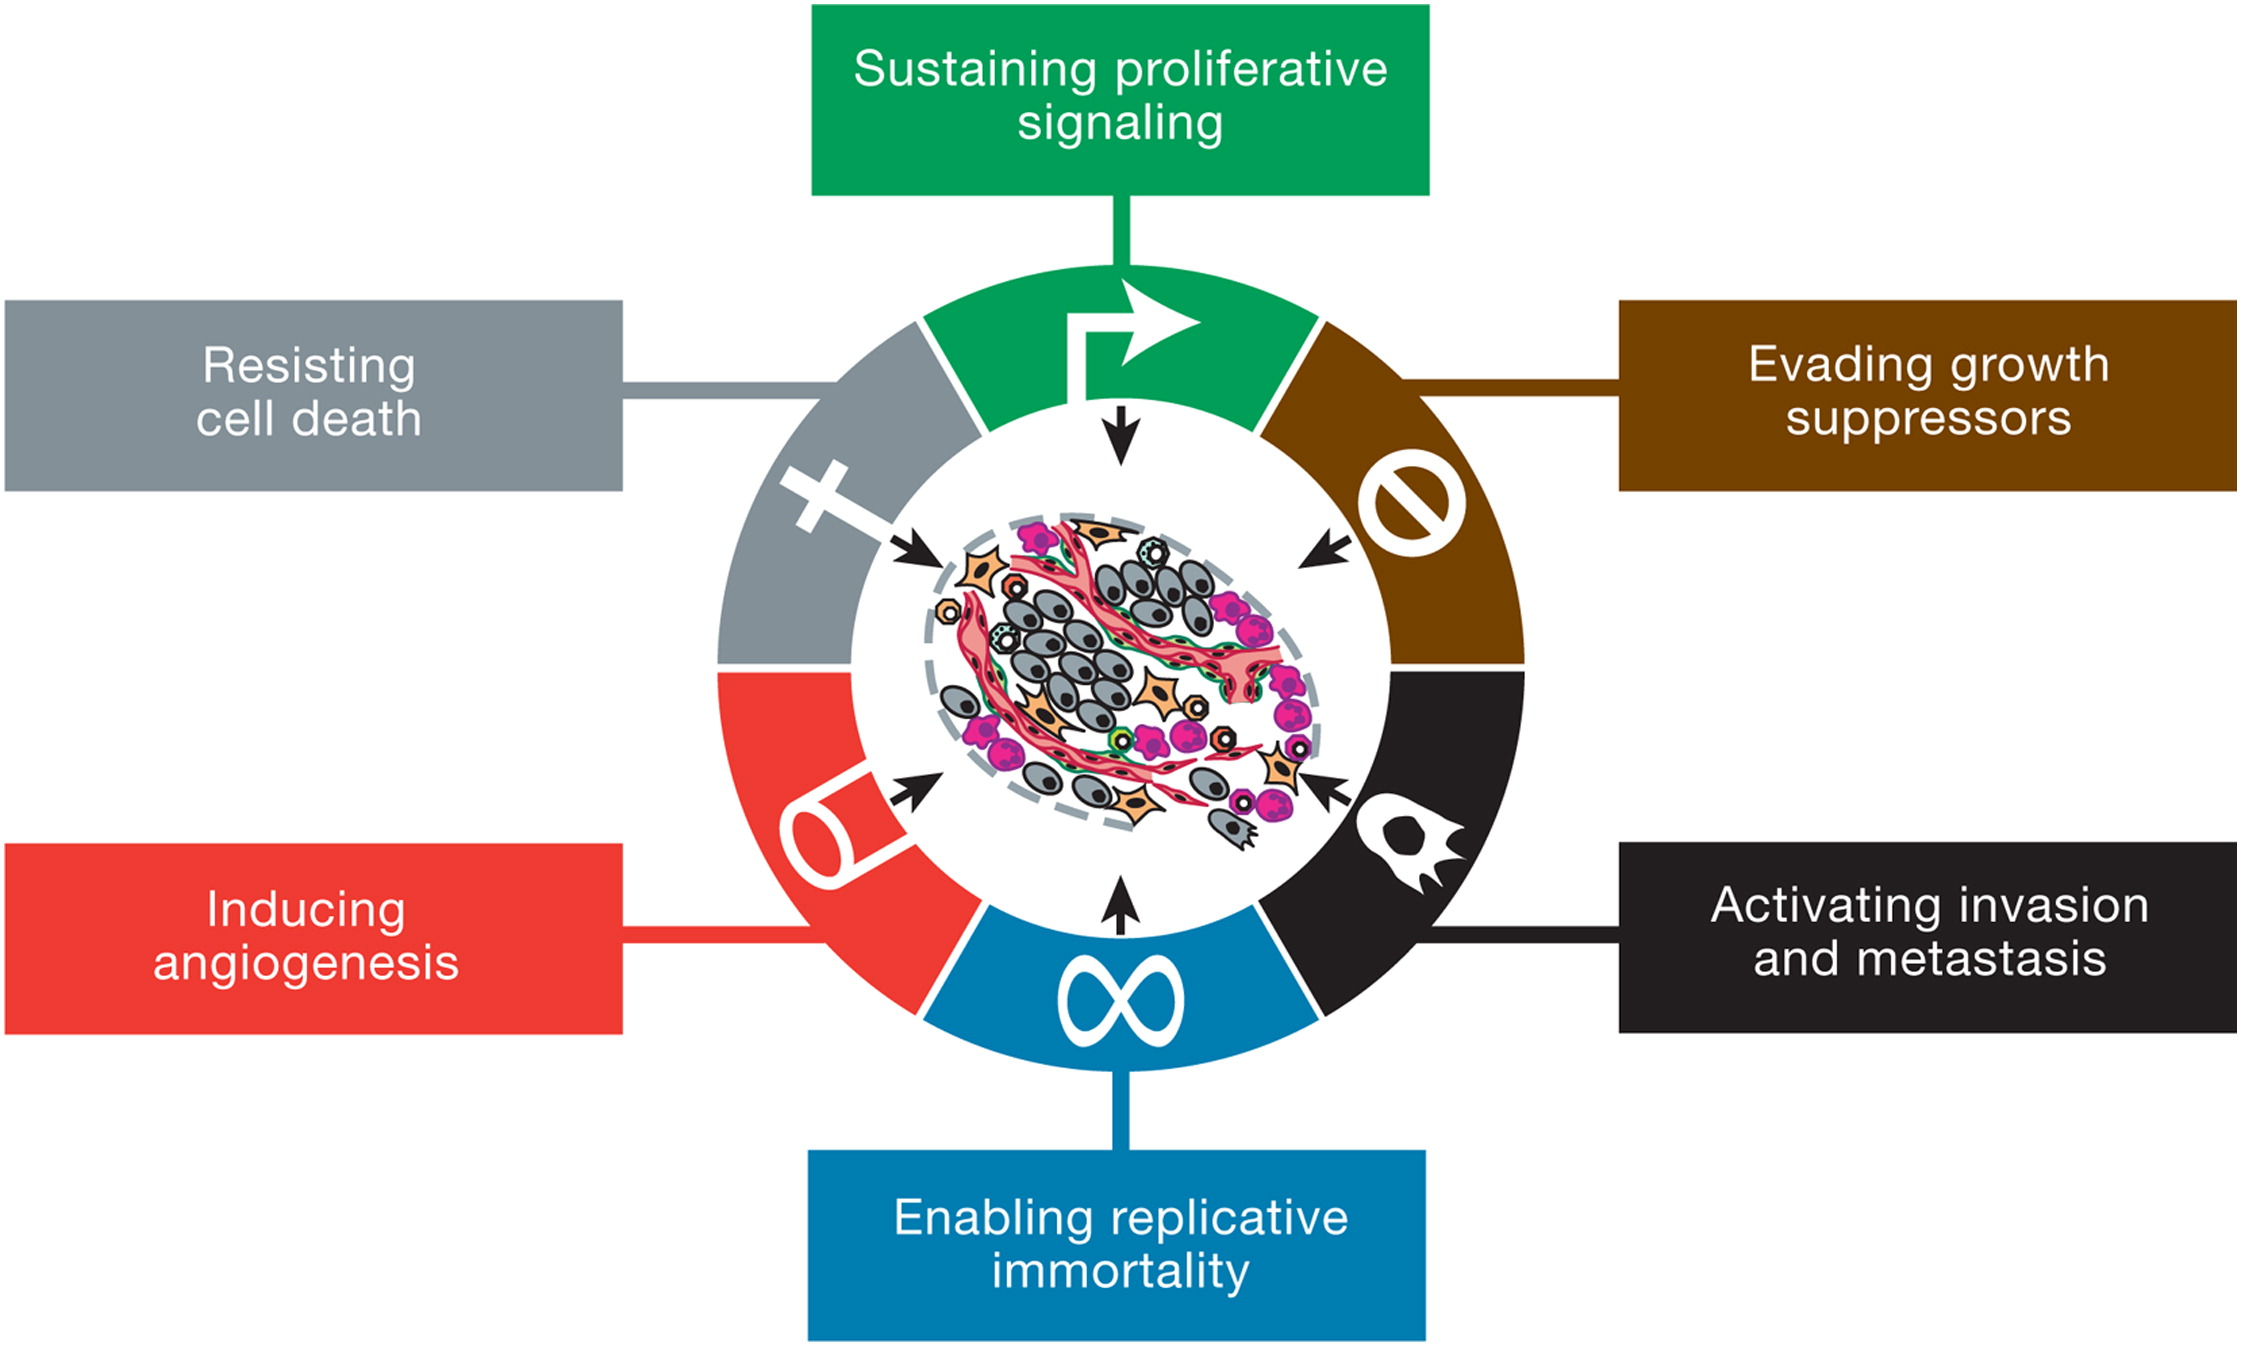
\includegraphics[width=0.45\textwidth]{figures/hallmarks.jpg}
    \caption{Hallmarks of Cancer~\cite{hallmarks_of_cancer}}
\end{figure}

Since these hallmarks are acquired through evolution, studying the phylogenies of cancer cells can help inform how the cells acquired their abilities. Phylogenies are trees that trace the evolutionary history of a cell. In cancer phylogenics, trees are defined such that the nodes are ``clones''. Clones are defined as the genetic makeup of a population of cancer cells with common mutations. Studying cancer phylogenies can provide insight into tumor behaviors and open new avenues for potential treatments. 

\subsection{CNA-Based Phylogenies}

Different kinds of mutations affect the genome to different magnitudes. The most commonly studied kinds of mutations in cancer phylogenetics are Single Nucleotide Variants (SNVs) and Copy Number Aberrations (CNAs). SNVs are when a single base pair in the DNA is erroneously changed, inserted, or deleted. Meanwhile, CNAs are when large geographical regions of base pairs are erroneously duplicated or deleted. 

\begin{figure}[ht]\label{fig:mutation_freq}
    \centering
    \includegraphics[width=0.45\textwidth]{figures/base_pair_mutations.png}
    \caption{Different kinds of mutations affect genomes differently and their effects are sometimes of vastly different scales. This graphic relates different kinds of mutations to the scale of base pairs affected by a mutation of that type.~\cite{lecture_2}}
\end{figure}

Researchers use genetic sequencing technologies to determine the state of SNVs and CNAs in a cell. The technology used determines what kind of analysis can be done with the data. If a technology has high coverage and low depth, it is considered optimal for determining SNVs in a cell. Meanwhile, if a technology has low coverage and high depth, it is considered optimal for determining the copy number state of a cell. There are currently no high-throughput technologies that provide sufficient data to do both SNV and CNA analysis. Therefore most approaches are geared towards one or the other. The CNT and ZCNT models that are discussed in this paper will focus on CNAs. 

There are two main phylogenetic problems to be solved: the Large Parsimony Problem and the Small Parsimony Problem. Large Parsimony is when you are given the copy-number states of cells and aim to organize them into a rooted evolutionary tree wherein every cell has exactly one parent. Meanwhile, Small Parsimony is when you are given the copy-number states of ``leaf-node'' cells and aim to generate the intermediary nodes of the phylogenetic tree. 

The core principle behind cancer phylogeny reconstruction is that mutations are rare~\cite{mutations_rare}. That means that in order to reconstruct cancer phylogenies, it is useful to define distance functions representative of the number of mutations. These allow us to construct phylogenetic trees that would require few mutations to generate, encouraging parsimonious evolutionary trees. Both ZCNT and CNT define different algorithms to determine distance. 

\subsection{CNA-Based Distance Functions}

Both CNT and ZCNT models have mathematical definitions of events. In both models, events represent a copy-number aberration that affects copy number profile $p$ over a range of loci from $s$ to $t$ inclusive ($s \leq t$) by increasing or decreasing the copy number by 1 (denoted by $b \in \{+1, -1\}$). 

They also both define the concept of a ``transformation'' to be a series of events. For instance, given events $(e_1, \hdots, e_n)$, a transformation would be defined as $T(p) = e_n(\hdots(e_1(p)))$. Both models define the distance between two profiles to be the minimum number of events required to transform one profile into another ($\text{dist}(u, v) = \min_{T(u) = v} |T|$). Events in a transformation are commutative under ZCNT~\cite{zcnt_paper}.

\subsubsection{CNT}

\newcommand{\cnt}{\textbf{cnt}}
\newcommand{\zcnt}{\textbf{zcnt}}

{\bf Copy Number Event Formula}: ($c_{s, t, b}: \mathbb{Z}_+^n \rightarrow \mathbb{Z}_+^n$) 
\begin{equation}
    c_{s, t, b}{(p)}_i = \begin{cases}
        p_i + b & \text{if}~s \leq i \leq t~\text{and}~p_i \neq 0 \\ 
        p_i & otherwise
    \end{cases}
\end{equation}

Given two copy number profiles, it is not guaranteed that there will be a transformation from one to the other under the CNT model. For instance, given $u=[0,1]$ and $v=[1,0]$, $u$ would have to amplify a copy number from zero to one in order to transform it into $v$. In these cases, the distance is defined as $+\infty$. We will denote the CNT distance between two profiles $u$ and $v$ as $\cnt(u, v)$.

Due to the lack of symmetry in the CNT model, two common methods have been employed to create symmetric measures from CNT for various parsimony algorithms.\vspace{5pt}

Both these algorithms are centered around getting the CNT distance in both directions. Mean Correction is when you take the average of the distances between two profiles. Median Distance just takes the lower of the two distances.

\def\arraystretch{2}

\vspace{10pt}

\begin{tabular}{|c|c|}
    \hline
    {\bf Method} & {\bf Formula} \\  \hline \hline
    Mean Correction & $\frac{\cnt (u, v) + \cnt (v, u)}{2}$ \\ \hline
    Median Distance & $\min \{\cnt (u, v), \cnt (v, u)\}$ \\ \hline
\end{tabular}

\vspace{15pt}

Both of these definitions raise interesting questions about reachability. Mean Correction amplifies unreachability because if either $\cnt(u, v)$ or $\cnt(v, u)$ does not exist, the Mean Correction will yield $+\infty$. Meanwhile, Median Distance amplifies reachability because even if either $\cnt(u, v)$ or $\cnt(v, u)$ does not exist, Median Distance will yield a noninfinite number. 

Instead of using a distance with these constraints, it is common to use another kind of intermediary. Some papers use the {\it copy number triplet\/} (CN3) problem. Which aims to pick some intermediate profile $w$ that minimizes $\cnt(w, u) + \cnt (w, v)$~\cite{triplet_algorithm}. 

While CN3 provides symmetry, it comes at the cost of computational time. CNT distances can be computed in $O(n)$ time~\cite{linear_cnt} while the most optimal current algorithm for CN3 is $O(nB^7)$ where $B$ is the largest copy number in the input profiles~\cite{triplet_algorithm}. The benefit of using CN3 is that the value is symmetric and therefore works well with existing parsimony methods.

\subsubsection{ZCNT}

{\bf Zero-Agnostic Copy Number Event Formula} 

($c_{s, t, b}: \mathbb{Z}^n \rightarrow \mathbb{Z}^n$) 

\begin{equation}
    c_{s, t, b}{(p)}_i = \begin{cases}
        p_i + b & \text{if } s \leq i \leq t \\ 
        p_i & otherwise
    \end{cases}
\end{equation}

Notice that the only difference between the ZCNT and CNT models is the removal of the non-negativity constraint in the function signature and the condition to skip $p_i$ if $p_i$ is zero. We will denote the ZCNT distance between two profiles $u$ and $v$ as $\zcnt(u, v)$. Unlike CNT distance, ZCNT distance always exists as a non-infinite number. 

In {\it A zero-agnostic model for copy number evolution in cancer\/}~\cite{zcnt_paper}, they propose the following closed-form formula for ZCNT distance: 

\begin{equation} \label{eq:1}
    \zcnt(u, v) = \frac{1}{2} ||\Delta (u) - \Delta (v)||_1
\end{equation}

where $\Delta (p)$ denotes another linear transform called {\it delta mapping\/} ($\Delta: \mathbb{Z}^{n} \rightarrow \mathbb{Z}^{n + 1}$)

\begin{equation} \label{eq:2}
    \Delta {(p)}_i = \begin{cases}
        p_1 - 2 & \text{if } i=1 \\ 
        2 - p_n & \text{else if } i=n+1 \\
        p_i - p_{i-1} & otherwise
    \end{cases}
\end{equation}

Due to ZCNT being the composition of two linear equations (Equations~\ref{eq:1} and~\ref{eq:2}), ZCNT can trivially be seen as an $O(n)$ algorithm. 